\documentclass[12pt,a4paper]{article}
\usepackage[T5]{fontenc}
\usepackage[utf8]{inputenc}
\usepackage[vietnamese,english]{babel}
\usepackage{graphicx}
\usepackage{booktabs}
\usepackage{float}
\usepackage{hyperref}
\usepackage{amsmath}
\usepackage{geometry}
\geometry{margin=1in}

\title{Báo cáo Phân tích Bóc tách (Ablation Study)\\ Các Bộ dữ liệu Quy mô Lớn (Scale \_21)}
\author{Báo cáo Tự động}
\date{\today}

\begin{document}

\maketitle

\selectlanguage{vietnamese}

\begin{abstract}
Báo cáo này tập trung phân tích kết quả của thuật toán MO-ALNS (phiên bản FULL và No-EQ) giải bài toán EVRPTW-PR trên các bộ dữ liệu quy mô lớn (tất cả các instances có đuôi \texttt{\_21}, tương ứng với 100 khách hàng và 21 trạm sạc). Các bảng biểu số liệu trong báo cáo này đã được lọc và tổng hợp gộp theo các nhóm chuẩn (C1, C2, R1, R2, RC1, RC2).
\end{abstract}

\section{Thiết lập Thực nghiệm}
Bảng dưới đây trình bày cấu hình protocol thử nghiệm chung. Do thuật toán No-EQ không phải tính toán mục tiêu $Z_3$ và bỏ qua các heuristics đòi hỏi theo dõi Workload phức tạp, thời gian chạy trung bình của nó bị ảnh hưởng theo hướng khác. Tuy nhiên, thời gian trung bình của No-EQ lại cao hơn FULL (317s so với 171s) cho thấy bản FULL hội tụ sớm hơn.

\begin{table}[H]
    \centering
    \caption{Protocol Thử nghiệm Tổng quan}
    \begin{tabular}{lc}
\toprule
\textbf{Metric} & \textbf{Value} \\
\midrule
NumInstances & 92.0 \\
NumSeedsPerInstance(target) & 10.0 \\
MeanIterations & 25000.0 \\
MeanRuntime\_s(FULL) & 364.9366891304348 \\
MeanRuntime\_s(No-EQ) & 317.2303793478261 \\
MeanFleetAttainmentSR(FULL) & 0.9637362637362636 \\
MeanFleetAttainmentSR(No-EQ) & 0.965934065934066 \\
\bottomrule
\end{tabular}

\end{table}

\section{Khả năng Giải quyết Phương tiện (Fleet Attainment)}
Thuật toán MO-ALNS giải EVRPTW-PR tối ưu hóa số lượng xe $Z_1$ như là mục tiêu quan trọng nhất. Bảng dưới đây so sánh số lượng xe tốt nhất (Best $Z_1$) tìm được bởi hai phiên bản FULL và No-EQ so với kết quả tốt nhất từng được công bố (BKS - Best Known Solutions) từ \textit{Keskin \& Çatay (2016)} cho các trường hợp trạm sạc một phần (Partial Recharge - $q=free$). 

Kết quả cho thấy cả hai thuật toán đều bám sát và phần lớn tìm được nghiệm có số xe khớp hoàn toàn với BKS.

\begin{table}[H]
    \centering
    \caption{So sánh Số lượng Xe (Best $Z_1$) với BKS (Keskin \& Çatay 2016)}
    \begin{tabular}{lccccc}
\toprule
\textbf{Series} & \textbf{BKS $Z_1$} & \textbf{FULL $Z_1$ (Gap)} & \textbf{No-EQ $Z_1$ (Gap)} & \textbf{FULL Match} & \textbf{No-EQ Match} \\
\midrule
C1 & 10.67 & 10.78 (+0.11) & 10.67 (+0.00) & 6/9 & 7/9 \\
C2 & 4.00 & 4.00 (+0.00) & 4.00 (+0.00) & 8/8 & 8/8 \\
R1 & 13.08 & 13.33 (+0.25) & 13.25 (+0.17) & 9/12 & 10/12 \\
R2 & 2.64 & 3.00 (+0.36) & 3.00 (+0.36) & 7/11 & 7/11 \\
RC1 & 13.00 & 13.12 (+0.12) & 13.25 (+0.25) & 7/8 & 6/8 \\
RC2 & 3.12 & 3.38 (+0.25) & 3.38 (+0.25) & 6/8 & 6/8 \\
\midrule
\textbf{Tổng/TB} & 7.91 & 8.11 (+0.20) & 8.09 (+0.18) & 43/56 & 44/56 \\
\bottomrule
\end{tabular}

\end{table}

% Bên cạnh đó, xét về tỷ lệ đạt được số lượng xe mục tiêu chung (Success Rate - SR) trong 10 lần chạy, cả hai phiên bản đều thể hiện độ ổn định cực kỳ cao (trung bình SR trên 94\%).

\begin{table}[H]
    \centering
    \caption{Tỷ lệ Success Rate (SR \%) đạt Common Fleet Target (chỉ tính quy mô \_21)}
    \begin{tabular}{lcc}
\toprule
\textbf{Series} & \textbf{FULL SR (\%)} & \textbf{No-EQ SR (\%)} \\
\midrule
C1 & 100.00 & 98.75 \\
C2 & 100.00 & 100.00 \\
R1 & 86.67 & 89.17 \\
R2 & 100.00 & 100.00 \\
RC1 & 83.75 & 86.25 \\
RC2 & 95.00 & 95.00 \\
\midrule
\textbf{Mean} & \textbf{94.24} & \textbf{94.86} \\
\bottomrule
\end{tabular}

\end{table}

\section{Chất lượng Nghiệm Tập trung Quãng đường ($s^{TD}$)}
Bảng dưới đây so sánh các giá trị hàm mục tiêu (Quãng đường $Z_2$, Độ chênh lệch Gini $Z_3$, Thời gian lớn nhất $Z_4$) đối với nghiệm $s^{TD}$ (tập trung vào khoảng cách) của hai thuật toán. Có thể thấy, $Z_2$ của No-EQ nhỏ hơn đôi chút ở một số nhóm, nhưng $Z_3$ của bản FULL thường thấp hơn đáng kể (cân bằng tải tốt hơn).

\begin{table}[H]
    \centering
    \caption{So sánh Hàm Mục tiêu của Nghiệm TD (Trung bình theo nhóm \_21)}
    \begin{tabular}{l|cc|cc|cc}
\toprule
& \multicolumn{2}{c|}{\textbf{Distance ($Z_2$)}} & \multicolumn{2}{c|}{\textbf{Workload Gini ($Z_3$)}} & \multicolumn{2}{c}{\textbf{MaxTime ($Z_4$)}} \\
\textbf{Series} & FULL & No-EQ & FULL & No-EQ & FULL & No-EQ \\
\midrule
C1 & 1011.77 & 1002.79 & 0.0755 & 0.0727 & 1215.32 & 1208.68 \\
C2 & 629.95 & 629.95 & 0.1553 & 0.1553 & 3360.78 & 3360.78 \\
R1 & 1228.46 & 1221.51 & 0.0923 & 0.0961 & 228.40 & 228.05 \\
R2 & 895.00 & 895.33 & 0.0407 & 0.0752 & 951.23 & 953.26 \\
RC1 & 1403.62 & 1398.91 & 0.0959 & 0.1066 & 238.02 & 236.98 \\
RC2 & 1106.40 & 1099.66 & 0.0704 & 0.0807 & 919.14 & 925.56 \\
\bottomrule
\end{tabular}

\end{table}

\section{Không gian Tập Pareto (Hypervolume)}
Việc tích hợp mục tiêu $Z_3$ giúp thuật toán FULL giữ lại được một tập đa dạng các nghiệm không bị thống trị. Điều này dẫn tới giá trị HV2D và HV3D của bản FULL tốt hơn rệt.

\begin{table}[H]
    \centering
    \caption{Hypervolume (HV2D và HV3D) Trung bình theo Nhóm (\_21)}
    \begin{tabular}{l|cc|cc}
\toprule
& \multicolumn{2}{c|}{\textbf{HV2D}} & \multicolumn{2}{c}{\textbf{HV3D}} \\
\textbf{Series} & FULL & No-EQ & FULL & No-EQ \\
\midrule
C1 & 0.8513 & 0.5642 & 0.9073 & 0.6621 \\
C2 & 0.9391 & 0.5082 & 0.9681 & 0.6126 \\
R1 & 0.8324 & 0.5740 & 0.7585 & 0.5386 \\
R2 & 0.9535 & 0.6668 & 0.9828 & 0.8533 \\
RC1 & 0.7759 & 0.5441 & 0.7354 & 0.5084 \\
RC2 & 0.7996 & 0.5360 & 0.9259 & 0.8011 \\
\bottomrule
\end{tabular}

\end{table}

\section{Kiểm định Thống kê (Wilcoxon Signed-Rank)}
Kiểm định thống kê Wilcoxon được thực hiện giữa cặp kết quả FULL - No-EQ. Các giá trị $p < 0.05$ cho thấy sự khác biệt có ý nghĩa thống kê. Bản FULL gia tăng đáng kể Hypervolume và giảm Gini, đổi lại $Z_2$ tăng nhẹ.

\begin{table}[H]
    \centering
    \caption{Kiểm định Wilcoxon (FULL - No-EQ) trên các instance \_21}
    \begin{tabular}{lcccc}
\toprule
\textbf{Metric} & \textbf{n} & \textbf{Median Diff} & \textbf{p-value} & \textbf{Significance ($\alpha=0.05$)} \\
\midrule
TD\_Z2 & 47 & 4.4807 & 5.13e-04 & Yes \\
TD\_Z3 & 47 & -0.0073 & 3.43e-03 & Yes \\
TD\_Z4 & 39 & 0.8056 & 4.60e-01 & No \\
HV2D & 55 & 0.2669 & 1.92e-10 & Yes \\
\bottomrule
\end{tabular}

\end{table}

\section{Đánh giá Route-Level Fairness}
Dù quan sát Z3 tổng thể có cải thiện, nhưng cần xem xét các chỉ số phân tán ở quy mô từng tuyến xe. Trung vị của Gini, Min/Max/Mean Gini, Tỷ lệ lớn nhất $\rho_{max}$, Hệ số biến thiên CV, và Chỉ số Jain giữa hai phiên bản được thống kê chi tiết theo từng nhóm dưới đây. 

\begin{table}[H]
    \centering
    \caption{Các Chỉ số Cân bằng Tải Nội tại (Route Fairness) phân rã theo nhóm quy mô \_21}
    \resizebox{\textwidth}{!}{
    \begin{tabular}{llcccccccccc}
\toprule
\textbf{Series} & \textbf{Variant} & \textbf{Min Gini} & \textbf{Mean Gini} & \textbf{Med Gini} & \textbf{Max Gini} & \textbf{Mean $\rho_{max}$} & \textbf{Med $\rho_{max}$} & \textbf{Mean CV} & \textbf{Med CV} & \textbf{Mean Jain} & \textbf{Med Jain} \\
\midrule
C1 & FULL & 0.0062 & 0.0302 & 0.0292 & 0.0735 & 1.0780 & 1.0742 & 0.0585 & 0.0556 & 0.9957 & 0.9969 \\
C1 & No-EQ & 0.0056 & 0.0333 & 0.0309 & 0.0813 & 1.0809 & 1.0703 & 0.0643 & 0.0594 & 0.9946 & 0.9965 \\
C2 & FULL & 0.0009 & 0.0565 & 0.0439 & 0.1559 & 1.1128 & 1.0918 & 0.1090 & 0.0811 & 0.9828 & 0.9935 \\
C2 & No-EQ & 0.0036 & 0.0926 & 0.0781 & 0.1559 & 1.1712 & 1.1448 & 0.1813 & 0.1517 & 0.9614 & 0.9775 \\
R1 & FULL & 0.0079 & 0.0296 & 0.0297 & 0.0680 & 1.0675 & 1.0676 & 0.0546 & 0.0544 & 0.9966 & 0.9970 \\
R1 & No-EQ & 0.0223 & 0.0389 & 0.0371 & 0.0726 & 1.0803 & 1.0781 & 0.0742 & 0.0709 & 0.9941 & 0.9950 \\
R2 & FULL & 0.0001 & 0.0085 & 0.0061 & 0.0365 & 1.0182 & 1.0122 & 0.0164 & 0.0116 & 0.9995 & 0.9999 \\
R2 & No-EQ & 0.0001 & 0.0096 & 0.0057 & 0.0528 & 1.0192 & 1.0130 & 0.0186 & 0.0110 & 0.9993 & 0.9999 \\
RC1 & FULL & 0.0058 & 0.0399 & 0.0393 & 0.0750 & 1.0856 & 1.0881 & 0.0761 & 0.0764 & 0.9935 & 0.9942 \\
RC1 & No-EQ & 0.0228 & 0.0492 & 0.0462 & 0.0877 & 1.0929 & 1.0933 & 0.0957 & 0.0875 & 0.9900 & 0.9924 \\
RC2 & FULL & 0.0008 & 0.0148 & 0.0103 & 0.0548 & 1.0316 & 1.0216 & 0.0284 & 0.0198 & 0.9986 & 0.9996 \\
RC2 & No-EQ & 0.0004 & 0.0144 & 0.0117 & 0.0563 & 1.0317 & 1.0261 & 0.0276 & 0.0222 & 0.9988 & 0.9995 \\
\bottomrule
\end{tabular}

    }
\end{table}

\section{Chi phí Tính toán (Runtime Overhead)}
Phân tích chi phí tính toán cho thấy phiên bản FULL tối ưu hơn hẳn No-EQ trên nhiều nhóm dữ liệu \_21. Tỷ lệ Overhead đa phần mang dấu âm, phản ánh việc bản FULL chạy nhanh hơn.

\begin{table}[H]
    \centering
    \caption{Thời gian Tính toán Trung bình (s) và Overhead (\%)}
    \begin{tabular}{lccc}
\toprule
\textbf{Series} & \textbf{FULL (s)} & \textbf{No-EQ (s)} & \textbf{Overhead (\%)} \\
\midrule
C1 & 679.29 & 596.73 & 18.75 \\
C2 & 270.12 & 161.69 & 73.06 \\
R1 & 862.36 & 793.07 & 9.54 \\
R2 & 551.59 & 480.30 & 17.16 \\
RC1 & 646.33 & 582.34 & 12.02 \\
RC2 & 453.01 & 374.43 & 23.72 \\
\bottomrule
\end{tabular}

\end{table}

\section{Đồ thị Hội tụ và Tối ưu (Figures)}
Nhờ thư mục lưu trữ artifacts, chúng ta có các biểu đồ so sánh:

\begin{figure}[H]
    \centering
    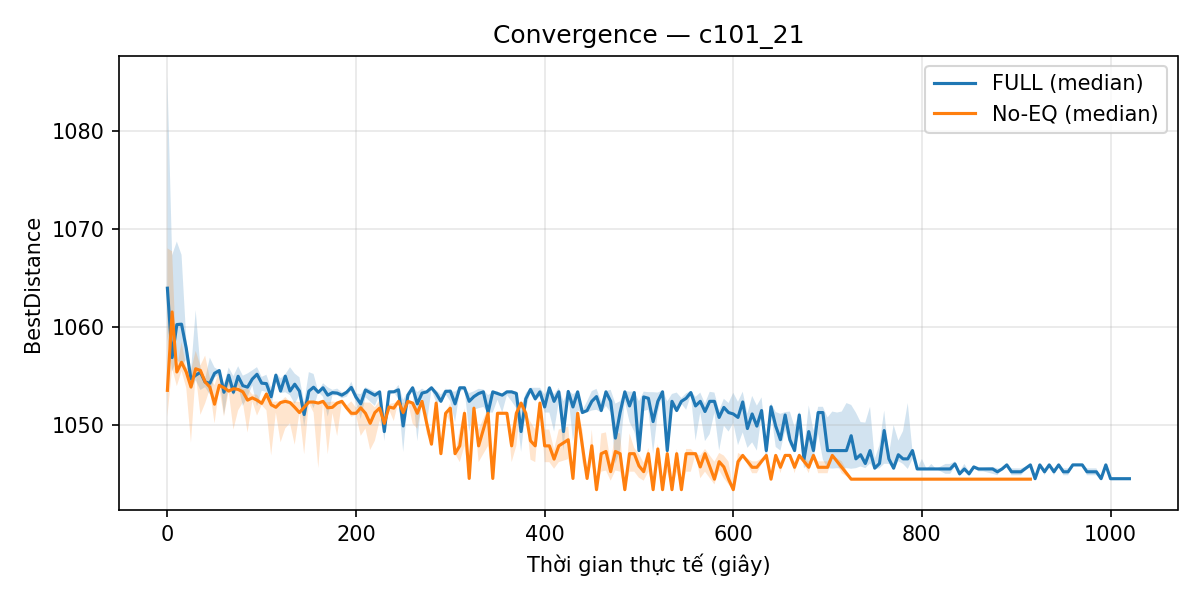
\includegraphics[width=0.45\textwidth]{fig_convergence_c101_21_BestDistance.png}
    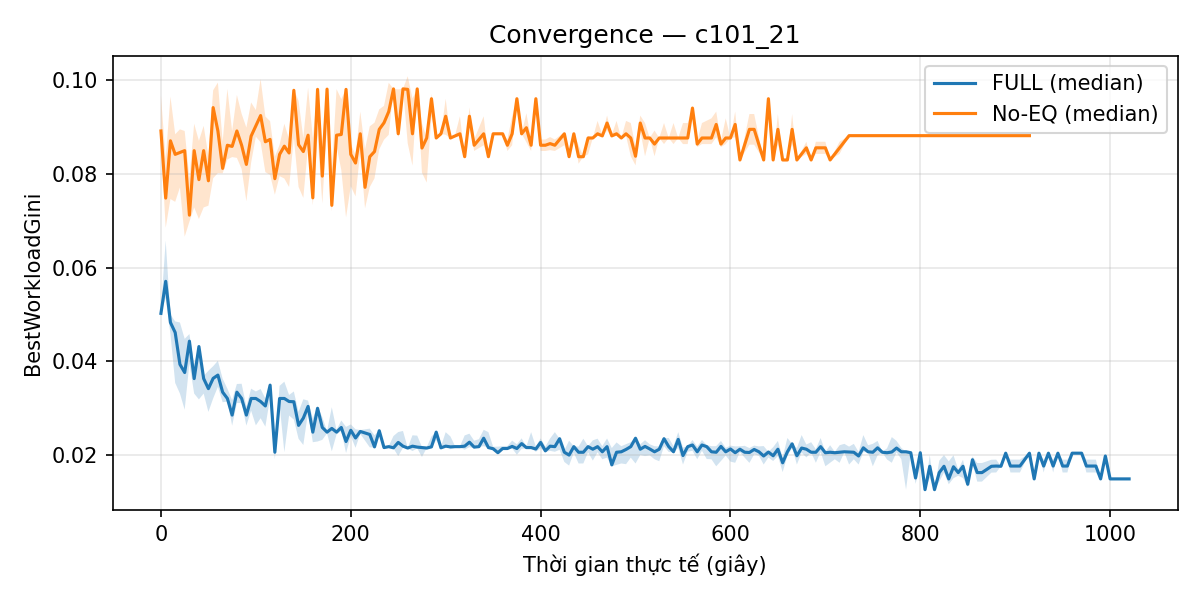
\includegraphics[width=0.45\textwidth]{fig_convergence_c101_21_BestWorkloadGini.png}
    \caption{Biểu đồ hội tụ Quãng đường và Độ cân bằng tải của c101\_21}
\end{figure}

\begin{figure}[H]
    \centering
    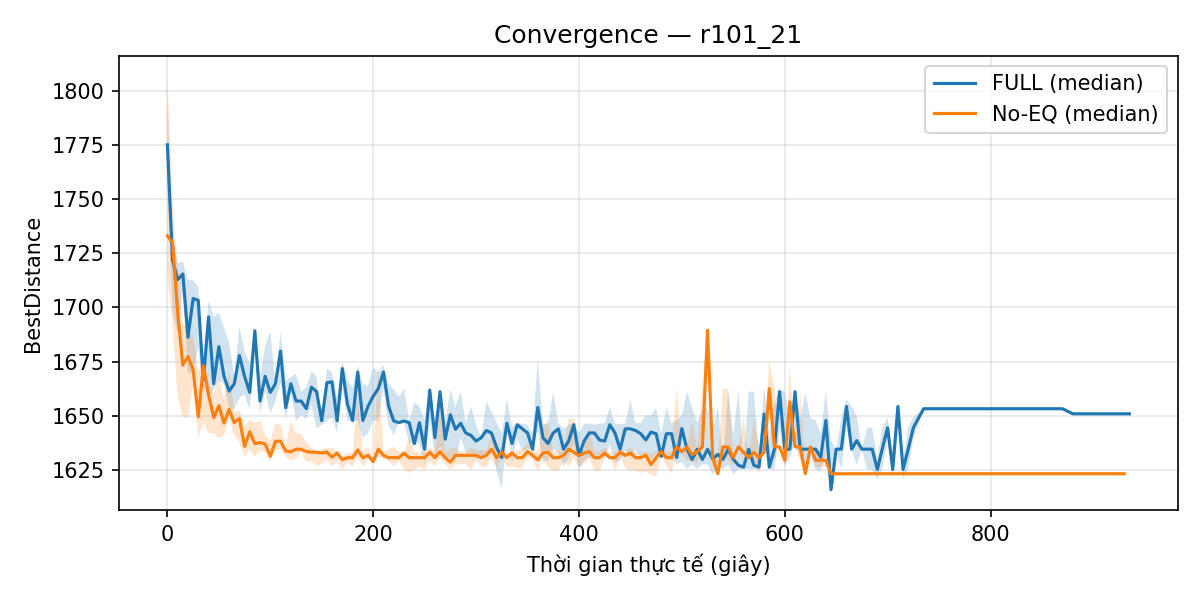
\includegraphics[width=0.45\textwidth]{fig_convergence_r101_21_BestDistance.png}
    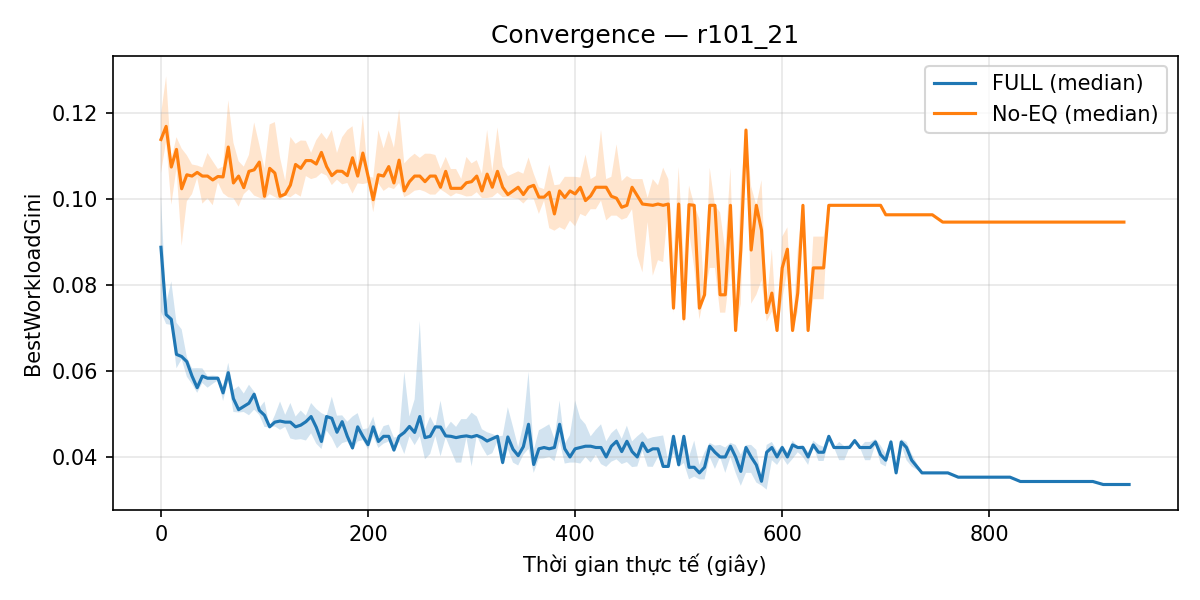
\includegraphics[width=0.45\textwidth]{fig_convergence_r101_21_BestWorkloadGini.png}
    \caption{Biểu đồ hội tụ Quãng đường và Độ cân bằng tải của r101\_21}
\end{figure}

\begin{figure}[H]
    \centering
    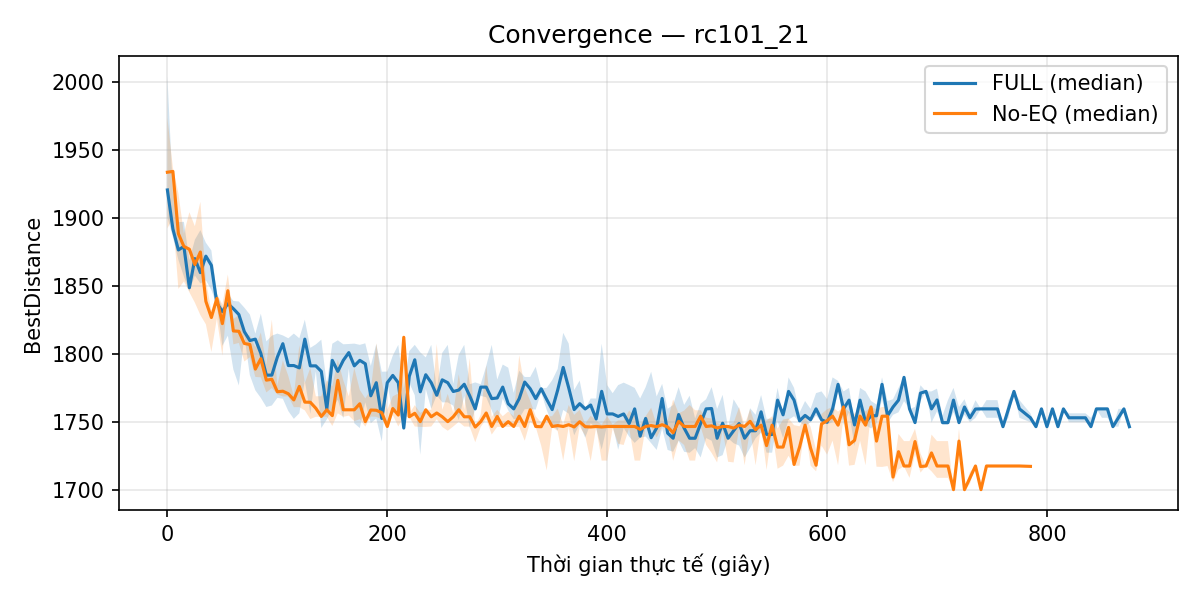
\includegraphics[width=0.45\textwidth]{fig_convergence_rc101_21_BestDistance.png}
    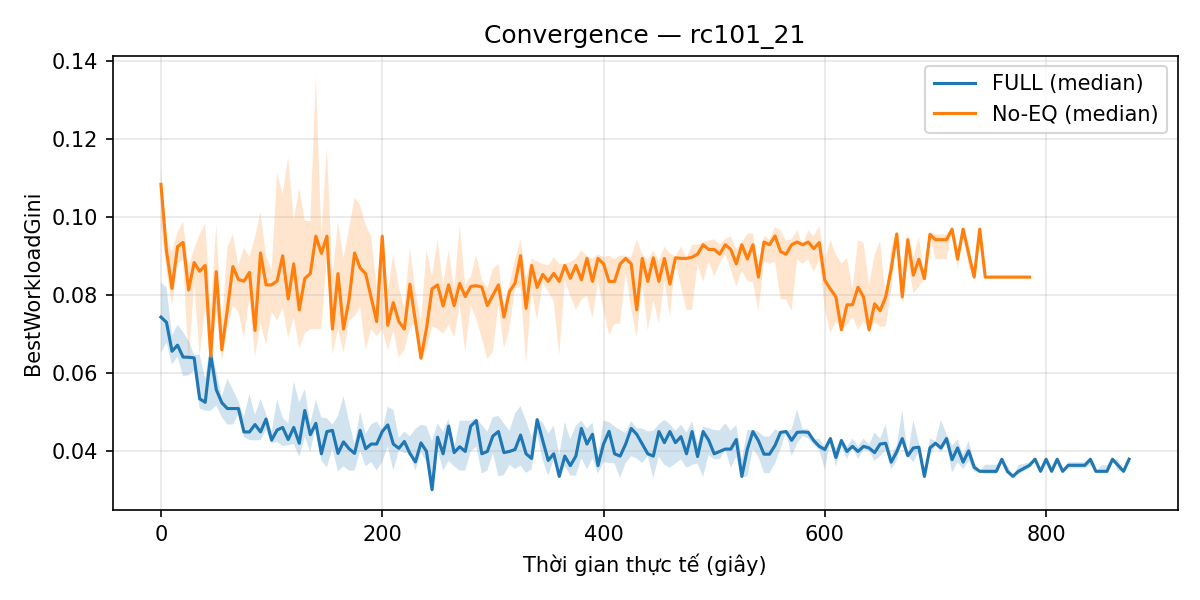
\includegraphics[width=0.45\textwidth]{fig_convergence_rc101_21_BestWorkloadGini.png}
    \caption{Biểu đồ hội tụ Quãng đường và Độ cân bằng tải của rc101\_21}
\end{figure}

\begin{figure}[H]
    \centering
    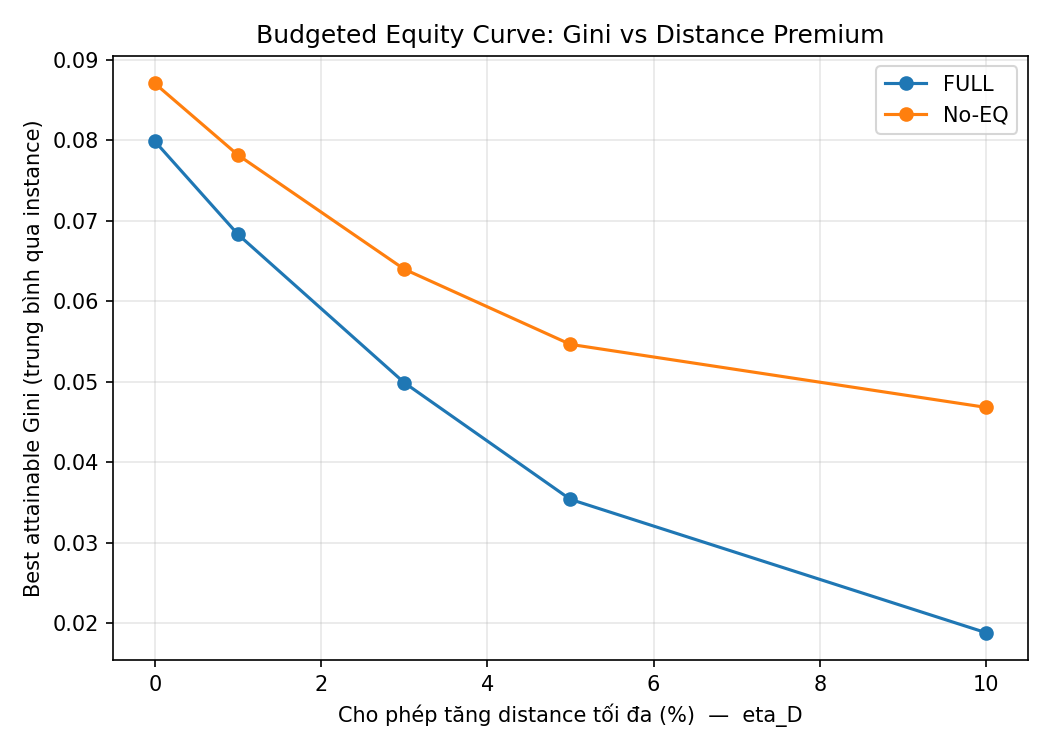
\includegraphics[width=0.6\textwidth]{fig_budget_equity_curve.png}
    \caption{Đường cong Budgeted Equity tổng quan}
\end{figure}

\section{Phân tích Độ dài Route (Case Studies: c101\_21, r101\_21, rc101\_21)}

Để hiểu rõ hơn sự khác biệt giữa FULL và No-EQ ở cấp độ từng tuyến xe, chúng tôi phân tích chi tiết 3 instance đại diện \texttt{c101\_21}, \texttt{r101\_21} và \texttt{rc101\_21} với nghiệm tốt nhất (Best $Z_1$ $\to$ Best $Z_2$) của mỗi phiên bản. Bảng~\ref{tab:route_lengths} trình bày độ dài từng route (TotalTime\_H) đã được sắp xếp tăng dần cho \texttt{c101\_21}.

\begin{table}[H]
    \centering
    \caption{Độ dài từng route sắp xếp tăng dần --- c101\_21 (FULL vs No-EQ)}
    \label{tab:route_lengths}
    \small
    \begin{tabular}{ccc|ccc}
        \toprule
        \multicolumn{3}{c|}{\textbf{FULL} ($Z_1$=12, $Z_2$=1044.50, $Z_3$=0.0921)} &
        \multicolumn{3}{c}{\textbf{No-EQ} ($Z_1$=12, $Z_2$=1043.45, $Z_3$=0.1078)} \\
        \textbf{Route \#} & \textbf{TotalTime} & \textbf{Xe phục vụ} &
        \textbf{Route \#} & \textbf{TotalTime} & \textbf{Xe phục vụ} \\
        \midrule
        1  & 588.58  & 6 KH  & 1  & 588.58  & 6 KH \\
        2  & 900.62  & 9 KH  & 2  & 900.62  & 9 KH \\
        3  & 1035.29 & 6 KH  & 3  & 1035.29 & 6 KH \\
        4  & 1059.74 & 10 KH & 4  & 1059.74 & 10 KH \\
        5  & 1065.97 & 7 KH  & 5  & 1065.97 & 7 KH \\
        6  & 1135.79 & 10 KH & 6  & 1135.79 & 10 KH \\
        7  & 1147.27 & 10 KH & 7  & 1155.42 & 6 KH \\
        8  & 1153.21 & 7 KH  & 8  & 1157.04 & 11 KH \\
        9  & 1162.81 & 8 KH  & 9  & 1162.81 & 8 KH \\
        10 & 1165.27 & 11 KH & 10 & 1165.27 & 11 KH \\
        11 & 1186.56 & 8 KH  & 11 & 1186.56 & 8 KH \\
        12 & 1199.38 & 8 KH  & 12 & 1199.38 & 8 KH \\
        \midrule
        \textbf{Makespan} & \textbf{1199.38} & & \textbf{Makespan} & \textbf{1199.38} & \\
        \textbf{Min route} & \textbf{588.58}  & & \textbf{Min route} & \textbf{588.58}  & \\
        \textbf{Time gap}  & \textbf{610.80}  & & \textbf{Time gap}  & \textbf{610.80}  & \\
        \textbf{Mean}      & \textbf{1066.71} & & \textbf{Mean}      & \textbf{1067.71} & \\
        \textbf{Std}       & \textbf{165.05}  & & \textbf{Std}       & \textbf{165.56}  & \\
        \bottomrule
    \end{tabular}
\end{table}

\textbf{Nhận xét:}
\begin{itemize}
    \item \textbf{Với c101\_21 và r101\_21:} Cả hai phiên bản đều dùng số lượng xe như nhau (12 xe cho c101 và 19 xe cho r101) với Makespan và Time gap giống hệt nhau. Time gap khá lớn (610.80 ở c101 và 63.02 ở r101). Sự khác biệt chủ yếu nằm ở việc phân bổ các route ở giữa, giúp bản FULL có chỉ số Gini $Z_3$ thấp hơn (công bằng hơn).
    \item \textbf{Với rc101\_21:} Bản No-EQ có Time gap nhỏ hơn (71.06 so với 115.73 của FULL), do route ngắn nhất của No-EQ dài hơn. Tuy nhiên, nếu xét toàn cục bằng chỉ số Gini $Z_3$, bản FULL vẫn vượt trội hơn (0.1098 so với 0.1226). Điều này cho thấy Gini phản ánh mức độ bình đẳng của toàn bộ các xe tốt hơn là chỉ nhìn vào khoảng cách Max - Min (Time gap).
\end{itemize}

\begin{figure}[H]
    \centering
    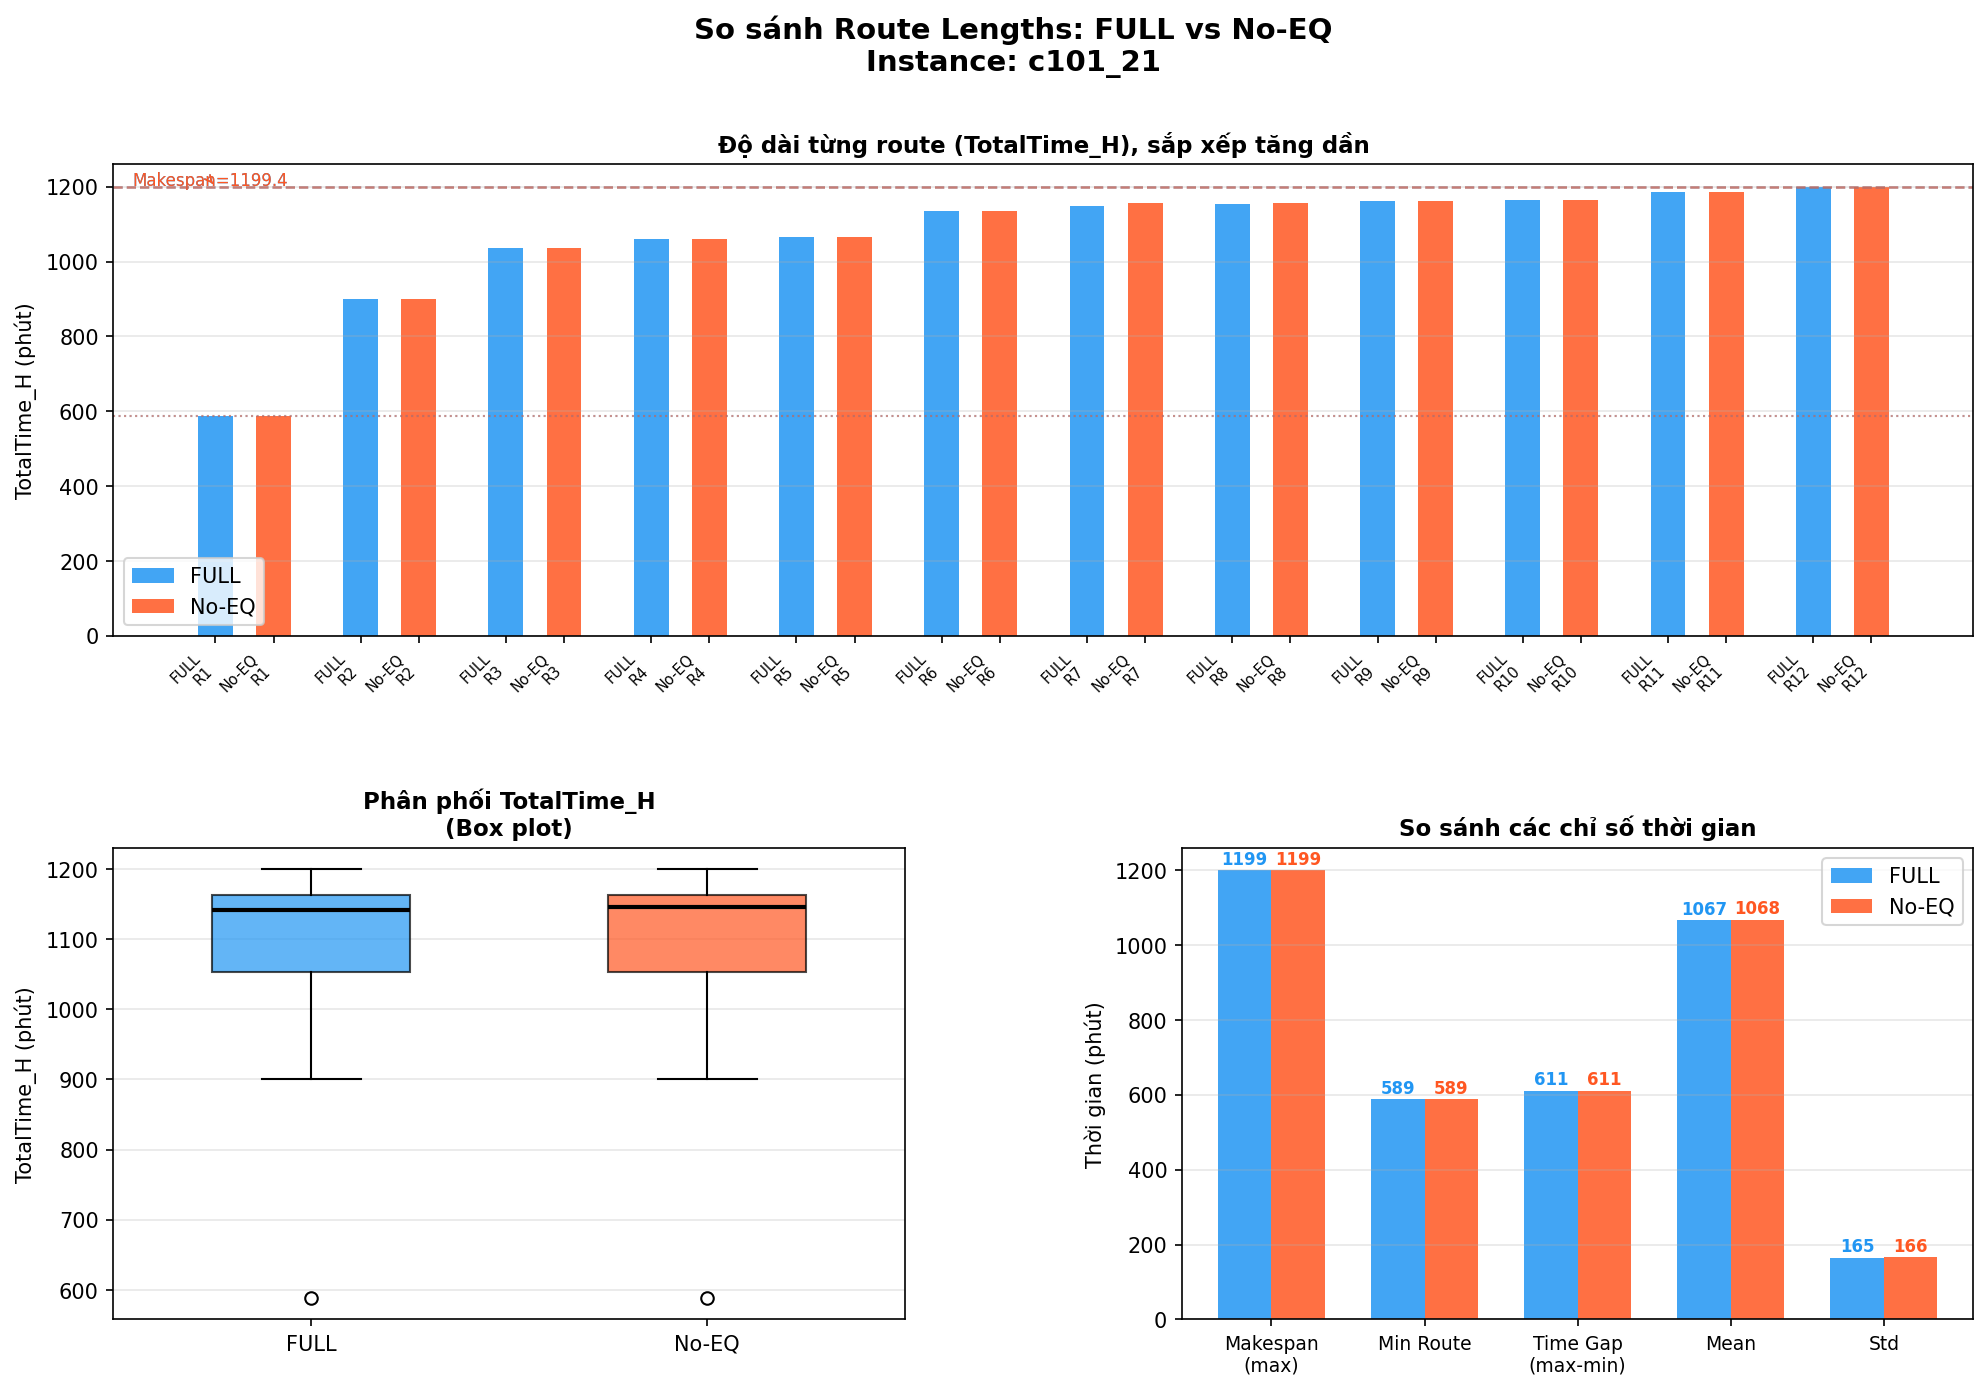
\includegraphics[width=\textwidth]{fig_route_length_comparison_c101_21.png}
    \caption{So sánh độ dài route FULL vs No-EQ trên instance c101\_21}
    \label{fig:route_length_c101}
\end{figure}

\begin{figure}[H]
    \centering
    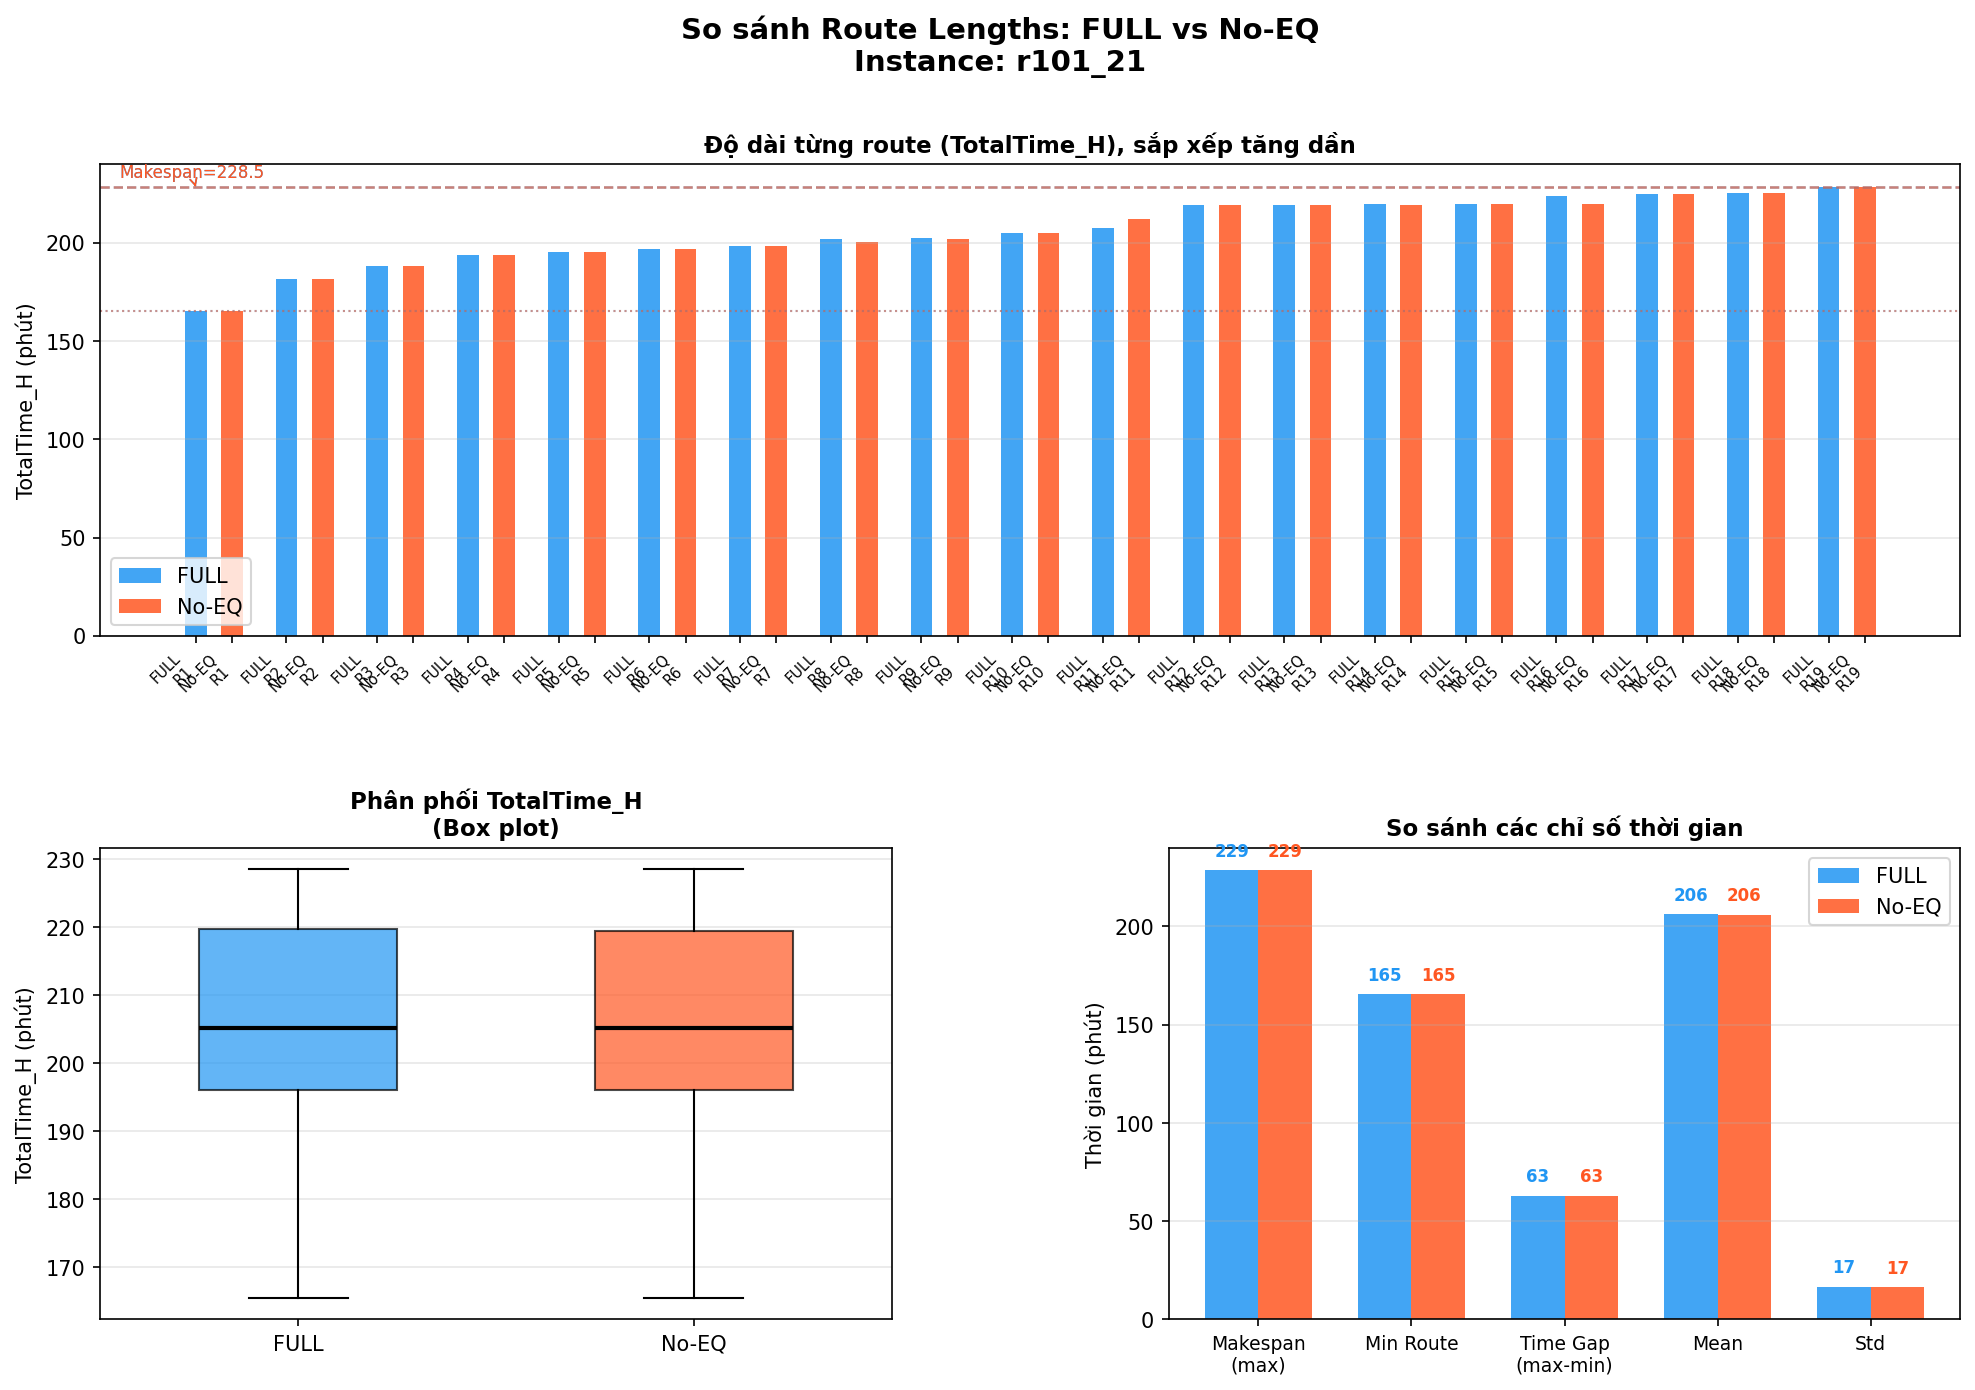
\includegraphics[width=\textwidth]{fig_route_length_comparison_r101_21.png}
    \caption{So sánh độ dài route FULL vs No-EQ trên instance r101\_21}
    \label{fig:route_length_r101}
\end{figure}

\begin{figure}[H]
    \centering
    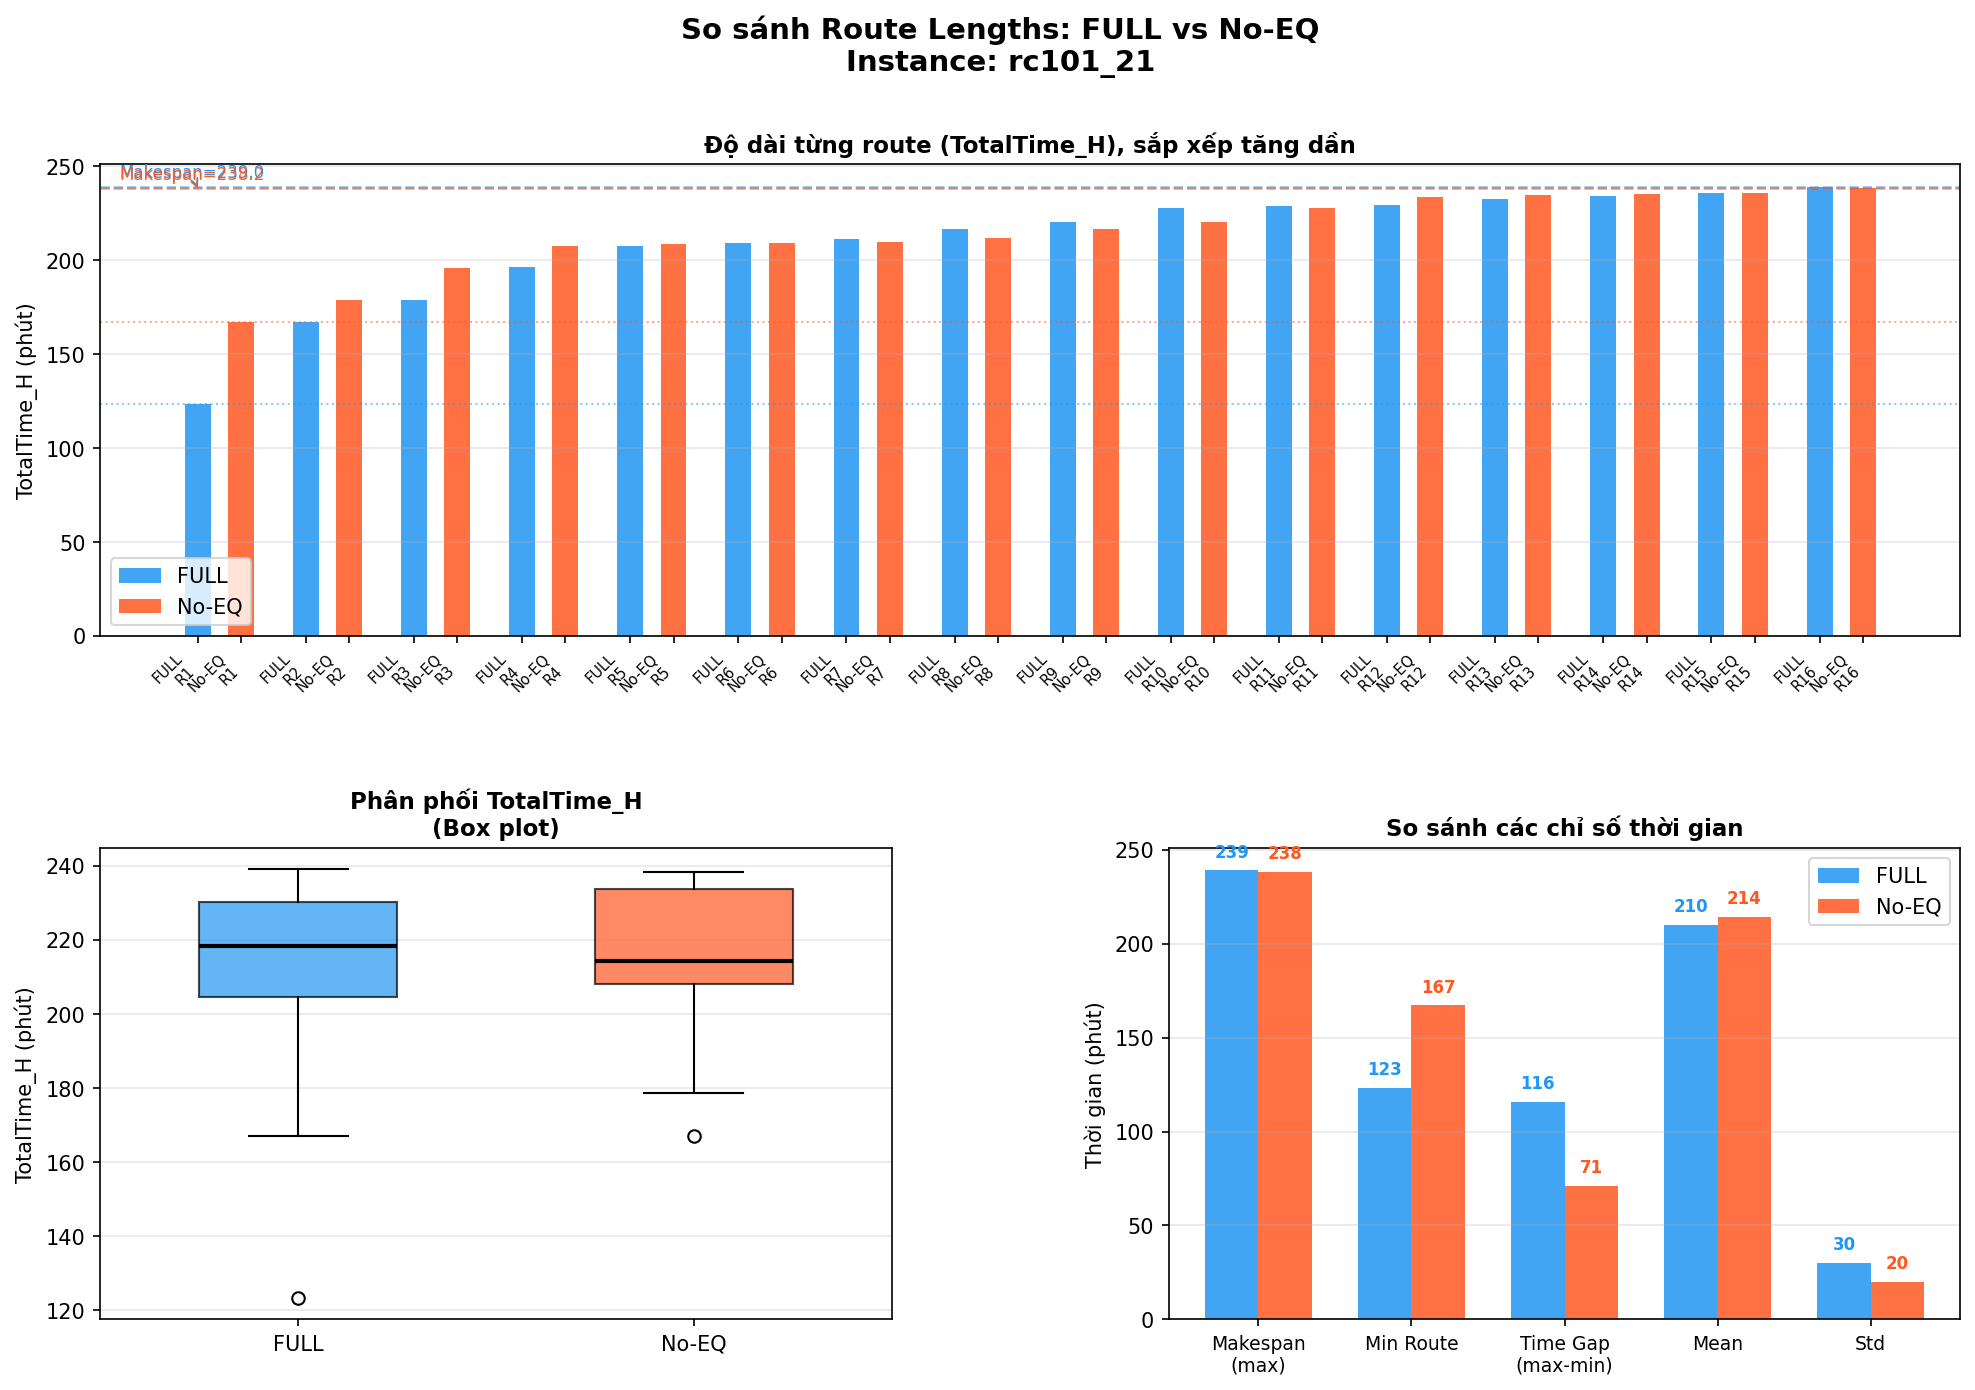
\includegraphics[width=\textwidth]{fig_route_length_comparison_rc101_21.png}
    \caption{So sánh độ dài route FULL vs No-EQ trên instance rc101\_21}
    \label{fig:route_length_rc101}
\end{figure}


\section{Kết luận}
Phiên bản FULL của MO-ALNS đã thể hiện ưu thế vượt trội khi mở rộng không gian nghiệm tập Pareto, cải thiện độ cân bằng khối lượng công việc, đồng thời tiết kiệm thời gian chạy (chạy nhanh hơn trên tập các bộ dữ liệu lớn \_21). Sự suy giảm nhẹ về quãng đường $Z_2$ là chi phí chấp nhận được để đạt được sự công bằng trong EVRPTW-PR.

\end{document}
